\chapter{Surrogate model for CFD}
\label{Surrogate model for CFD}
To develop a surrogate model which mimics the behaviour of CFD in finding the drag coefficient at zero degree angle of attack, it is essential to identify the limits of design parameters, perform Design Of Experiments (DOE) on them, perform CFD analysis at these DOE points and fit a surrogate model. The whole processes is described in the subsections below.

\section{Mapping design variables}
The first task before creation of DOE was the proper definition of the upper and lower limits for the six design variables (viz., $ m, r_0, r_1, C_p, \frac{l}{d} \ and \  scale \_y $). The upper and lower limits of design variables are calculated using the initial sizing done by Alam [\citenum{alam2017thesis}]. The design space is confined as mentioned in Table \ref{Degign space }

\begin{table}[H]
	\centering
	\caption{Design Space}
	\label{Degign space }
	%\begin{ruledtabular}
	\begin{tabular}{lll}
		\hline \hline
		Design Parameters & Min. & Max.    \\ \hline \hline
		
		$ Point\ of\ Max.\ Dia., m$ & 0.35 & 0.50     \\  
		$ Nose\ Radius, r _{o} $ & 0.20 & 0.80     \\
		$ Tail\ Radius, r _{1} $ & 0.1 & 0.5     \\  
		$ Prismatic\ Coeff., C _{p }$ & 0.55 & 0.70 \\
		$ Fineness\ Ratio, \frac{l}{d} $ &2.50 & 6.00 \\
		$Scaling\ in\ Y\ direction,\ scale\_y$ &1.00 & 3.00\\ \hline \hline
	\end{tabular}
	%	\end{ruledtabular}
\end{table}

Eighty candidate points were first obtained by Surrogates Toolbox \textbf{cite surrogate toolbox} using the Optimal Latin Hypercube Sampling (OLHS) method. The generated points were then mapped to the shapes corresponding to envelope having \textit{Reynolds number (Re)} of 3.01e6.

\section{Design of Experiments study}

As mentioned previously in Section \ref{DOE}, DOE study is used to extract maximum amount of information from every experiment conducted. This is especially needed when we are carrying out expensive computer or real life experiments. While developing surrogate model for CFD, each CFD analysis will take about 3 hours to complete. Hence to optimally use the computation resources, the total number experiments needs to be as low as possible but extracting maximum information about function behaviour. So, initially the number of experiments are taken as 80 and the design points are generated using the \textit{Optimal Latin Hypercube Sampling (OLHS)} technique present in SURROGATES Toolbox by Viana [\citenum{viana2014metamodeling}]. The obtained points are given in Appendix.


\section{Training data for CFD surrogate model}
\label{Training data CFD}
All the pre-processing required to perform CFD analysis like creating geometry, deciding grid size and meshing the domain has been automated using Octave and C++ scripting. In our case, 80 DOEs are generated and steady state 3D CFD analysis has been performed for these 80 shapes. The solver parameters used are as follows:
\begin{table}[H]
	\caption{Flow conditions and solver parameters for all DOE shapes}
	\label{Flow conditions and solver parametres for all DOE shapes}
	\centering
	\begin{tabular}{ll}
		\hline \hline
		Parameters & Value \\ 
		\hline \hline
		Reynolds number based on volume Re & $ 3.01 \ast 10^6 $ \\
		Pressure, ($ N/m^2 $) & 87500 \\
		Density, ($ Kg/m^3 $) & 1.057 \\
		Speed, ($ m/s $) & 51 \\
		Mesh & Hexahedral mesh using \textit{blockMesh} and \textit{snappyHexMesh} \\
		Solver & \textit{SimpleFOAM} (Incompressible steady state solver) \\
		Turbulent..? & Yes \\
		Turbulence model & K-Omega SST \\
		\hline \hline
	\end{tabular}
\end{table}
\section{Grid Convergence study}

Effect of grid size on the overall results by  changing the number of cells in self similar mesh has been carried out. Below is the plot of variation of pressure and viscous drag with number of cells for a simulation. As mentioned by Suman et al.[\citenum{Suman2011}] , when the percentage change in the values is less than 5 \%, then the solution is reported to have grid convergence.

\begin{table}[H]
	\caption{Grid convergence study}
	\label{Grid convergence table}
	\centering
	\begin{tabular}{ccc}
		\hline \hline
		Cells & Pressure Drag (N) & Viscous Drag (N) \\
		\hline \hline
		376380 & 1.1  & 11.02 \\
		604375  & 2.2  & 11.68 \\
		840565  & 2.02  & 12.1 \\
		994864  & 2.09  & 12.24 \\
		1563471  & 2.12 & 12.5 \\
		\hline \hline
	\end{tabular}
\end{table}

\begin{figure}[H]
	\centering
	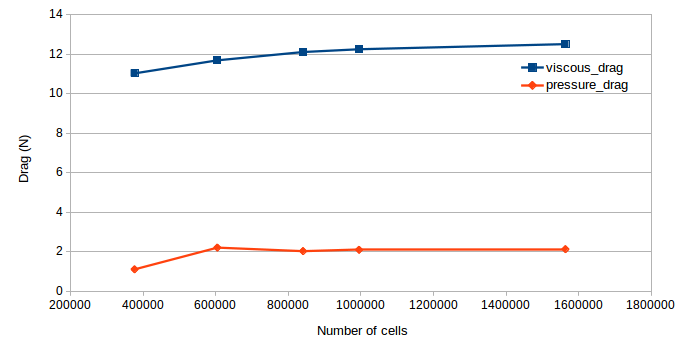
\includegraphics[width=300 pt]{surrogate_model_CFD_results/Grid_convergence.png}
	\caption{Variation of pressure and viscous drag with number of cells}
	\label{Grid convergence plot} %      only if needed
\end{figure}
Since there is no considerable amount of change in drag values, the number of cells are taken are around 1 million instead of 1.5 million for all the cases. This saves computational time.

\section{Results of CFD simulations}
\begin{figure}[H]
	\centering
	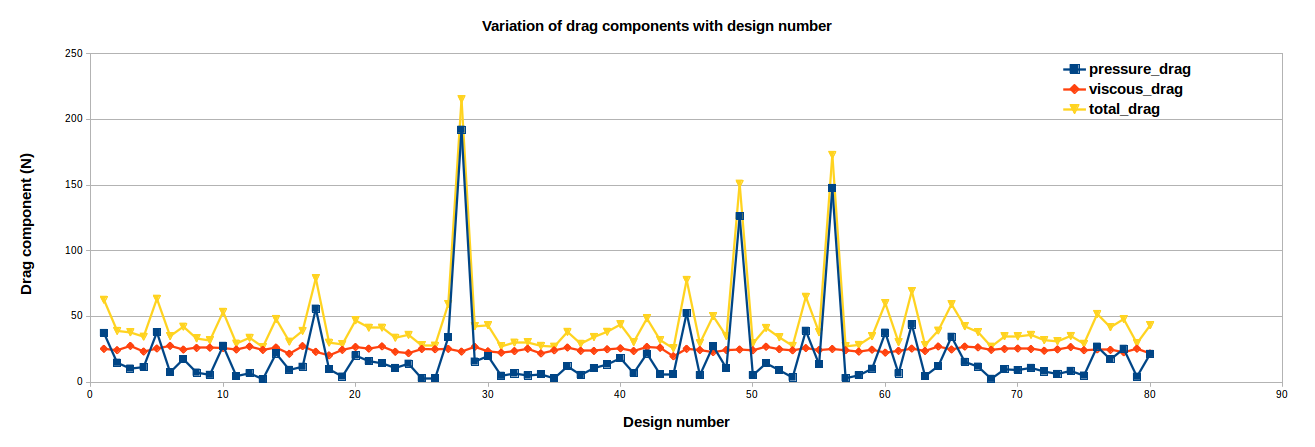
\includegraphics[width=450 pt]{surrogate_model_CFD_results/Drag_components.png}
	\caption{Variation of pressure and viscous drag with design number}
	\label{Drag components plot} %      only if needed
\end{figure}

\begin{figure}[H]
	\centering
	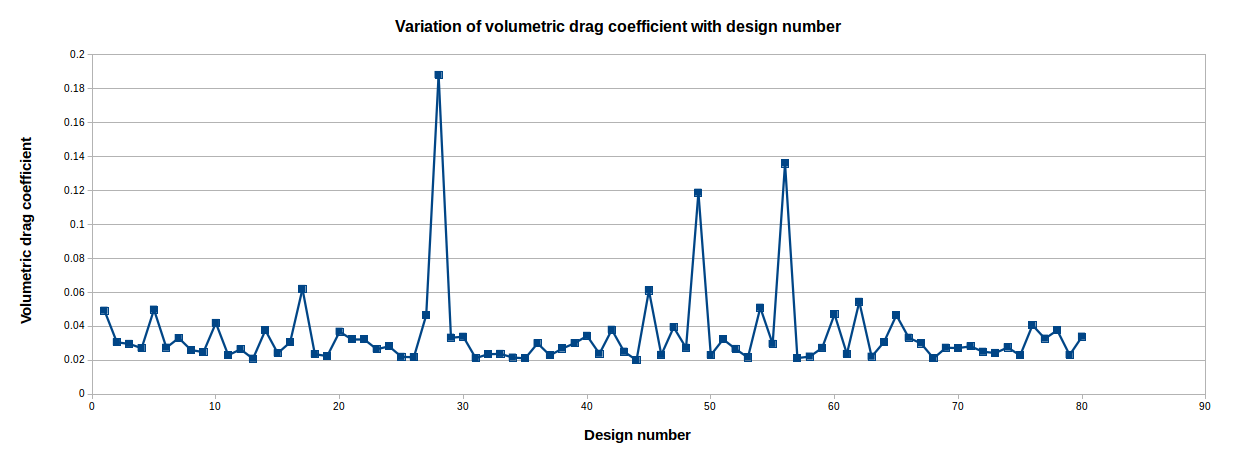
\includegraphics[width=450 pt]{surrogate_model_CFD_results/Volumetric_drag_coeff.png}
	\caption{Variation of volumetric drag coefficient with design number}
	\label{Volumetric drag coefficient plot} %      only if needed
\end{figure}

From Fig. \ref{Volumetric drag coefficient plot} we can see that some shapes are having very high drag coefficient compared to others. To see one of these high and low drag bodies visually, they have been drawn in Fig. \ref{visual comparison} one on top of other with scale being the same. Given a fixed volume, bodies with non-axisymmetric shapes will have higher frontal area compared to axisymmetric body as shown in Fig.\ref{visual comparison}. This makes the non-axisymmetric body more 'bluffy'. This leads to flow separation which is a non-linear phenomenon.

\begin{figure}[H]
	\centering
	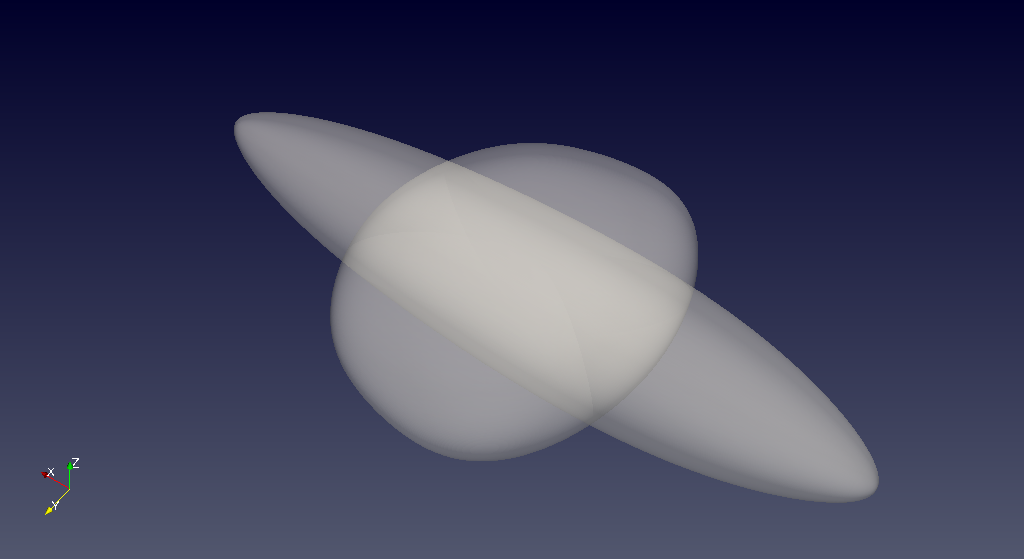
\includegraphics[width=300 pt]{rnd/visual_low_high.png}
	\caption{Visual comparison of low and high drag bodies}
	\label{visual comparison} %      only if needed
\end{figure}

The surface streamlines have been plotted in Figure \ref{low drag body} and \ref{high drag body} to understand the physics behind large difference in drag. It can be seen that long sleek body is having very less flow separation at the leading edge whereas the other body with more frontal area is have more flow separation and wake region.

\begin{figure}[H]
	\centering
	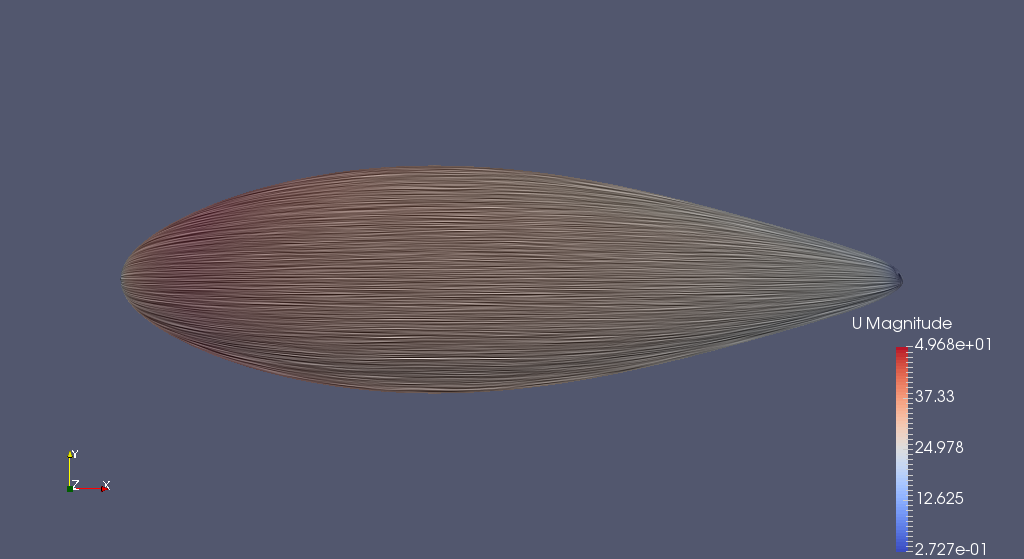
\includegraphics[width=300 pt]{rnd/streamlines_25_l.png}
	\caption{Surface streamlines on the body with low pressure drag}
	\label{low drag body} %      only if needed
\end{figure}

\begin{figure}[H]
	\centering
	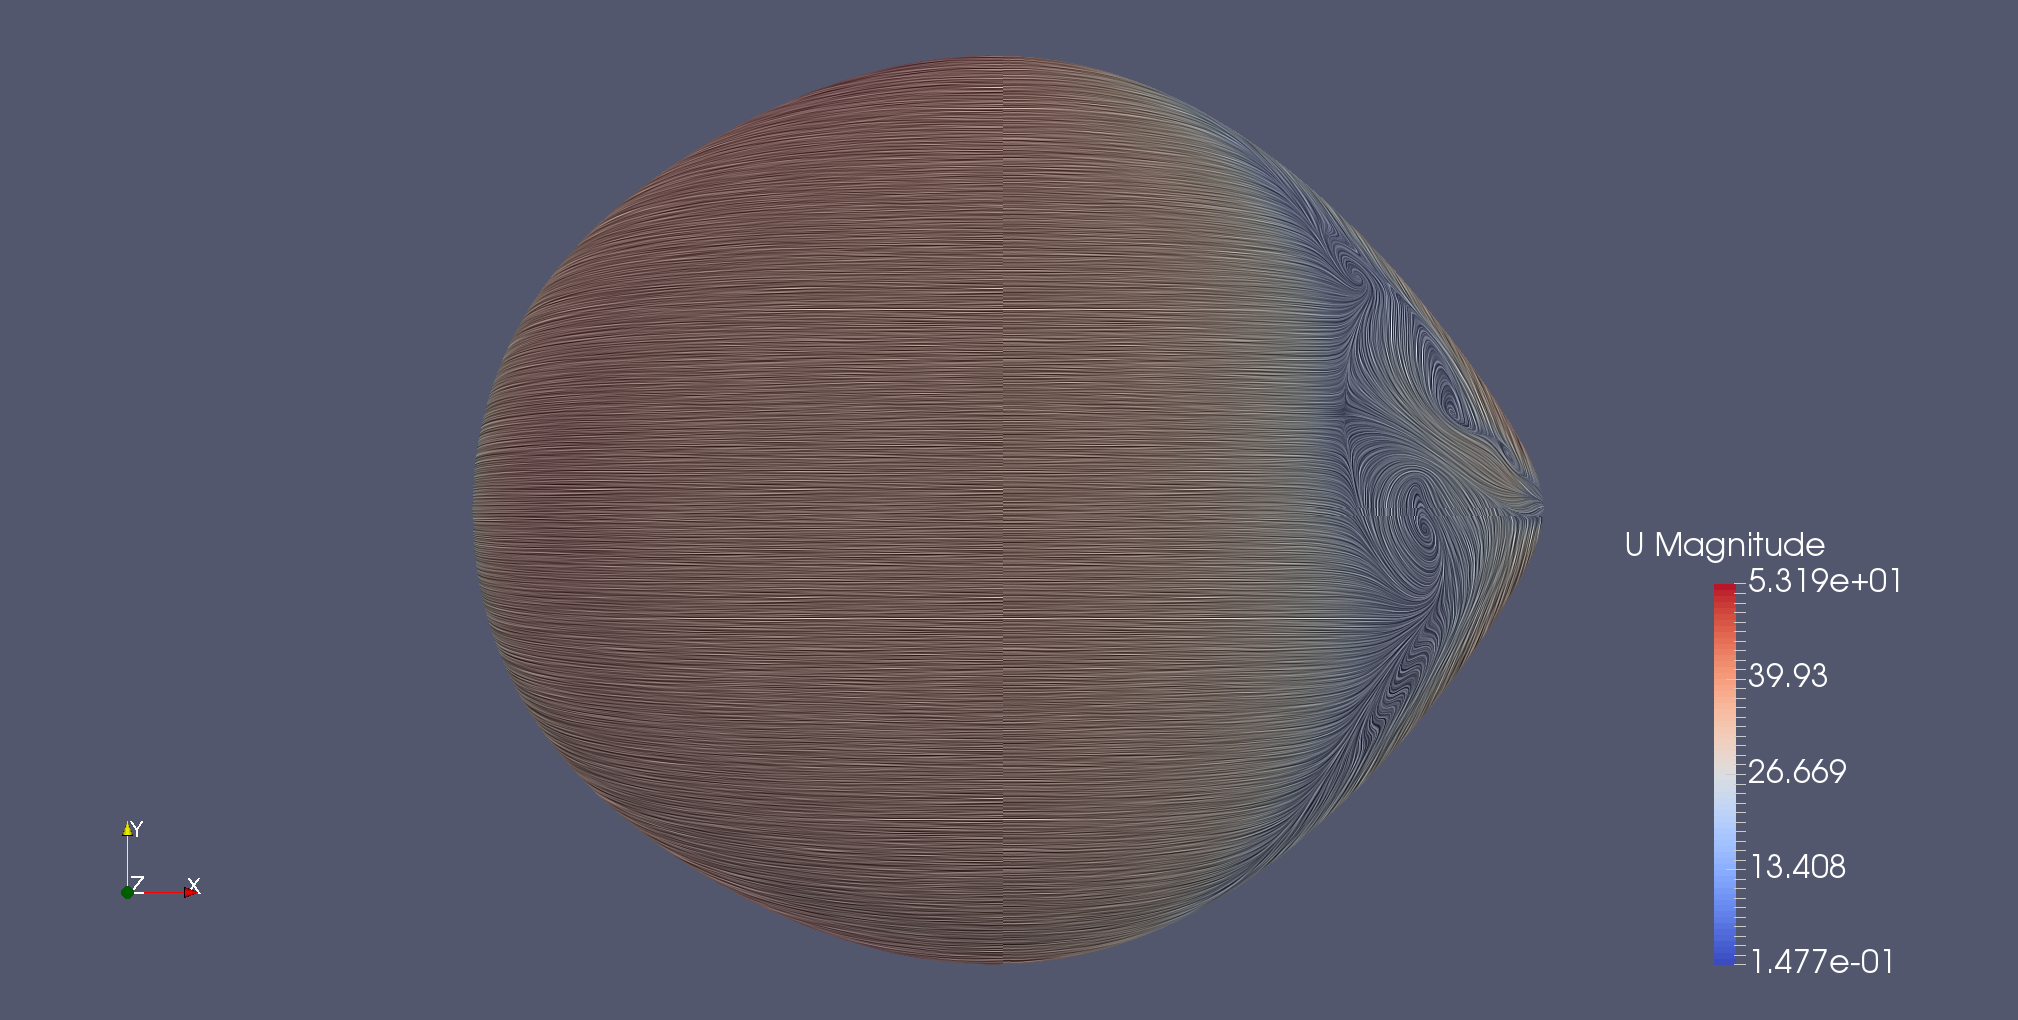
\includegraphics[width=300 pt]{rnd/streamlines_45.png}
	\caption{Surface streamlines on the body with high pressure drag}
	\label{high drag body} %      only if needed
\end{figure}

To couple a surrogate model with optimizer, the model needs to be accurate enough. The \% error should be less than 2\% as suggested by Alam[\citenum{alam2017thesis}]. But because of large variance in the training data, the model obtained is not accurate enough. This is because the bodies having more pressure drag because of flow separation are acting as outliers in the training data. So, the bodies having volumetric drag coefficient more than 0.04 are not considered while fitting the model. This gives a fairly better model with \% error $ \le $ 6\% in the case of Kriging.
Since the few bodies with higher drag are acting as outliers for the model, they are not considered while training the model. So, bodies with $ C_{DV} \ge 0.04$ are not considered in model building. To improve the accuracy of model, 40 more points are added to training set.

\begin{figure}[H]
	\centering
	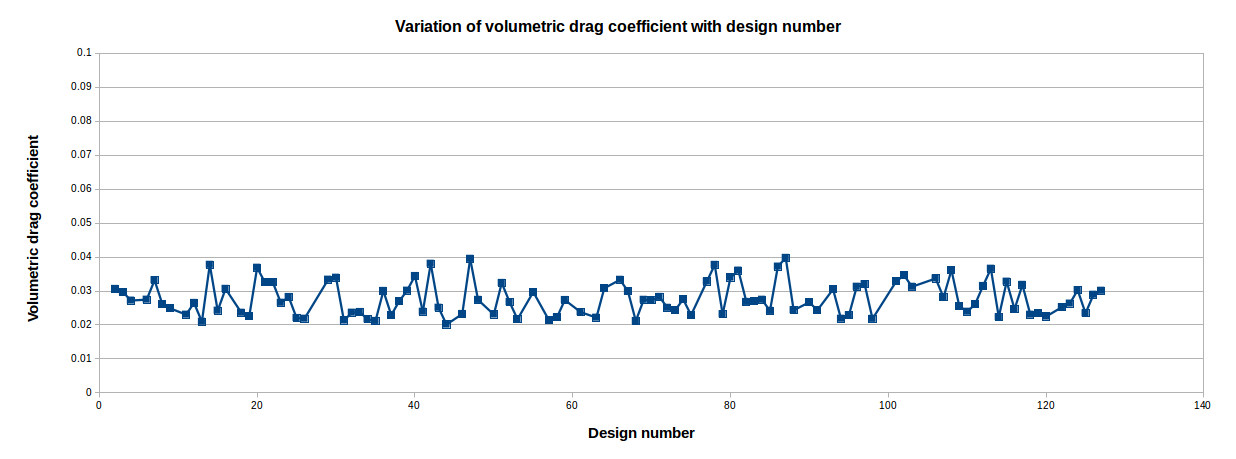
\includegraphics[width=450 pt]{surrogate_model_CFD_results/Volumetric_drag_coeff_training.png}
	\caption{Variation of volumetric drag coefficient with design number for training dataset}
	\label{Volumetric drag coefficient plot training data} %      only if needed
\end{figure}

\section{Testing the accuracy of surrogate model}

Three surrogate models mentioned in Section \ref{Different surrogates used during this investigation} has been fit to the above data. Then eight random design points has been generated in the domain for testing purpose. The results are shown in Table \ref{Accuracy of different surrogate models}.

\begin{table}[H]
	\caption{Accuracy of different surrogate models}
	\label{Accuracy of different surrogate models}
	\centering
	\begin{tabular}{cccc}
		\hline \hline
		Random Exp.No	&Kriging (\% Error)	&PRS (\% Error)	&RBF (\% Error) \\
		\hline \hline
		1 &5.72 &3.24	&2.73 \\
		2 &4.82	&11.33	&36.40 \\
		3 &0.96	&6.09	&12.73 \\
		4 &1.15	&7.98	&18.62 \\
		5 &2.50	&5.40	&14.13 \\
		6 &1.29	&6.31	&1.75 \\
		7 &1.99	&0.59	&10.05 \\
		8 &5.64	&3.36	&1.12 \\
		\hline \hline
		Avg. \% Error	& 3.00875	& 5.5375	& 12.19 \\
		\hline \hline
	\end{tabular}
\end{table}


From the above results we can observe that Kriging predicted the functional behaviour with more accuracy. RBF is having more error because the amount of training data to fit RBF is not sufficient in our case. Accuracy of polynomial response surface is between Kriging and Radial basis function. This is because PRS only sees at the global functional behaviour and under-fits the model. So, Kriging has been selected for coupling with optimizer in our study.

Also, few machine learning algorithms have been applied to see if they predict better than Kriging. It can be seen from Table \ref{Accuracy of different machine learning models} that none of them is predicting the functional behaviour better than Kriging. The reason is obvious as machine learning models are very generalized models and they can be used for both numerical and non-numerical experiments provided that large amount of training data is available. Since in our case the data is limited, we cannot use machine learning models. This further demonstrates the efficacy of Kriging for predicting functional behaviour of numerical experiments.
\begin{table}[H]
	\caption{Accuracy of different machine learning models}
	\label{Accuracy of different machine learning models}
	\centering
	\begin{tabular}{ccccc}
		\hline \hline
		\specialcell{ Random \\ Exp.No}	& \specialcell{Linear Regression \\ (\% Error)}	&\specialcell{Ridge Regression \\ (\% Error)}	& \specialcell{SVR \\ (\% Error)} & \specialcell{Kernel Ridge \\ (\% Error)} \\
		\hline \hline
		1 &4.89	&8.45	&48.86	&37.40 \\
		2 &22.60	&31.31	&74.30	&96.77 \\
		3 &31.62	&33.77	&77.00	&115.31 \\
		4 &20.15	&24.09	&74.03	&96.03 \\
		5 &15.34	&16.81	&45.69	&59.07 \\
		6 &11.67	&1.08	&27.72	&21.22 \\
		7 &12.90	&15.42	&48.52	&62.18 \\
		8 &1.68	&17.80	&64.92	&62.44  \\ 
		\hline \hline
		Avg. \% Error  &15.10	&18.59	&57.63	&68.80		 \\
		\hline \hline
	\end{tabular}
\end{table}








